% ============================================================
% 棋盘格 A4 版: 12x9 格 (内角 11x8), 方格 15mm (180x135mm)
% 打印: 100% 实际大小(不要"适应页面"), 标定参数: -s 15
% ============================================================
\documentclass{article}
\usepackage[a4paper, margin=8mm]{geometry}
\usepackage{tikz}
\pagestyle{empty}
\setlength{\parindent}{0pt}
\begin{document}
\begin{center}
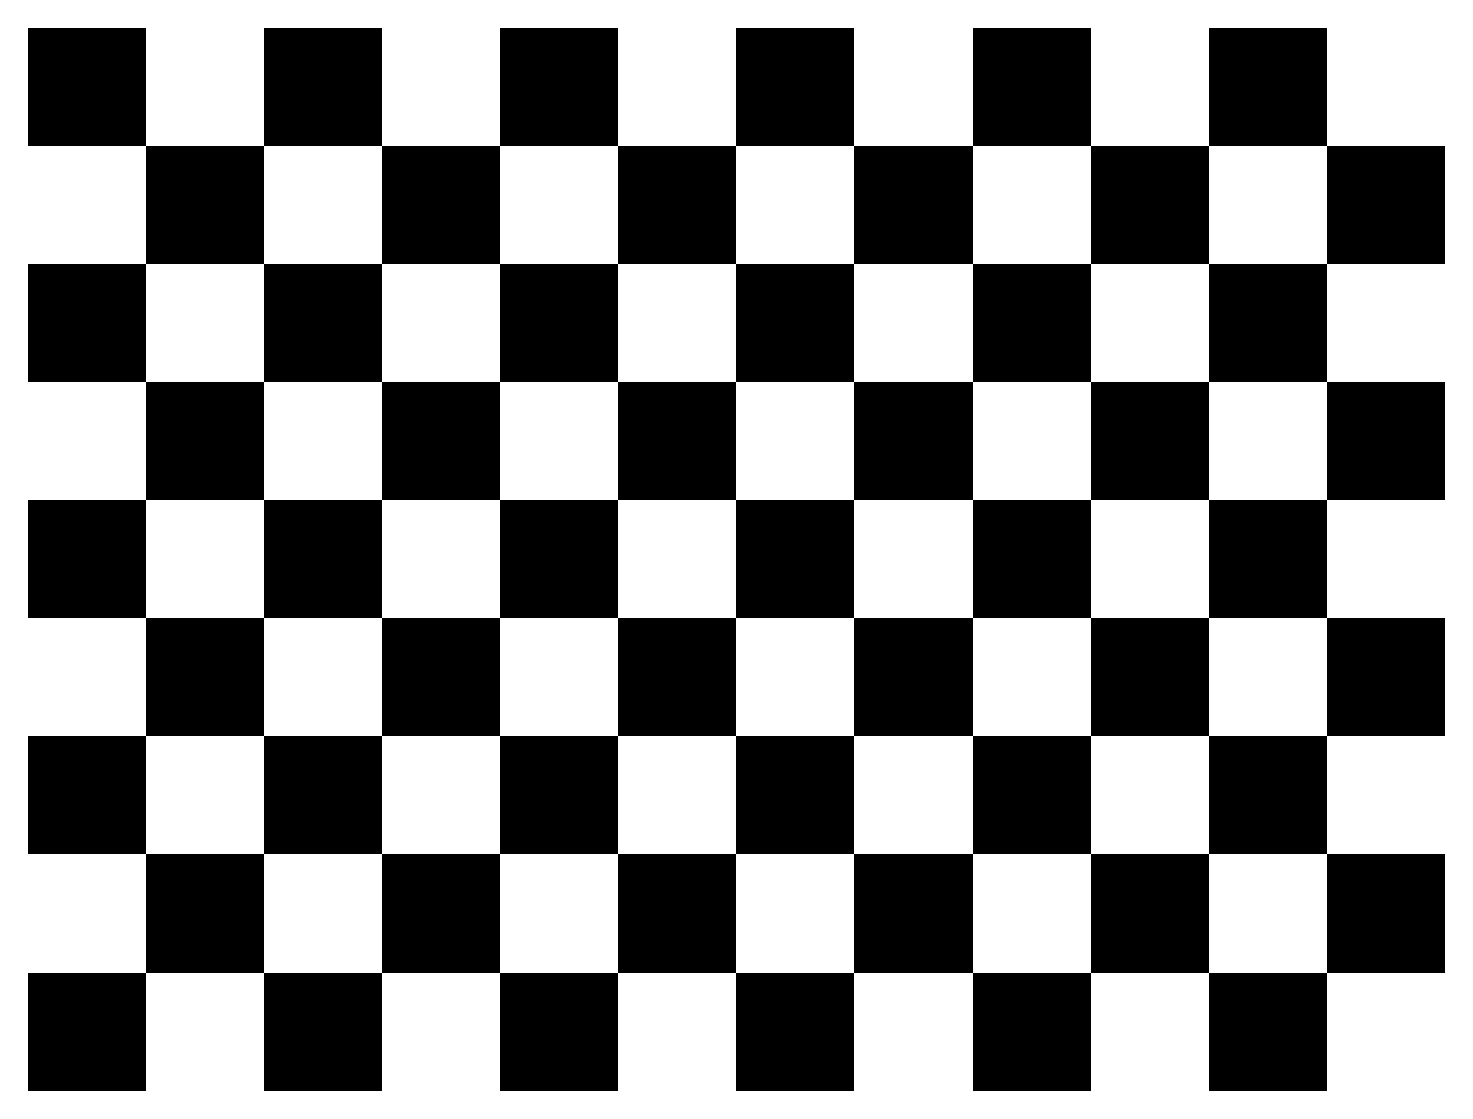
\begin{tikzpicture}
  \def\s{15mm} % 方格边长
  \foreach \row in {0,...,8}{
    \foreach \col in {0,...,11}{
      \pgfmathparse{int(mod(\row+\col,2))}
      \ifnum\pgfmathresult=0
        \fill[black] (\col*\s,-\row*\s) rectangle ++(\s,\s);
      \fi
    }
  }
\end{tikzpicture}

\vspace{3mm}
{\large Checkerboard: 12$\times$9 (11$\times$8 inner corners), square 15mm}\\[1mm]
{\small Print at 100\% actual size. Calibration: \texttt{-w 11 -h 8 -s 15}}
\end{center}
\end{document}
